\chapter{Сферический трехосный пассивный электростатический подвес} \label{chapt3}

% \section{Определение главного вектора сил и главного момента для сферического тела в электростатическом подвесе} \label{sect3_1}

% \section{Анализ жесткости электростатического подвеса для различной формы электродов}\label{sect3_2}

\section{Построение конечно-элементной модели трехосного пассивного электростатического подвеса} \label{sect3_1}

Объектом исследования является упрощенная схема трехосного электростатического подвеса, приведенная на рис. \ref{img:sphere_susp_scheme}. Построим конечно-элементную модель в программной системе ANSYS, принимая следующие допущения:
\begin{enumerate}
  \item Центр тяжести сферического ротора совпадает с его геометрическим центром
  \item Каналы X, Y, Z подвеса строго ортогональны друг другу
  \item Результирующая пондеромоторная сила каждого из каналов X, Y, Z в любой момент времени действует вдоль оси своего канала
  \item Моменты сил, действующих на ротор, отсутствуют
\end{enumerate}

С учетом введенных допущений конечно-элементную модель построим следующим образом: электрические цепи моделируем \textit{CIRCU124} элементами, сферический ротор представим точечным элементом массы \textit{MASS21}, емкости, образованные ротором и фиксированными обкладками каждого из каналов, моделируем электромеханическими элементами-преобразователями \textit{TRANS126}. На рис. представлена схема расчетная конечно-элементная схема трехосного пассивного электростатического подвеса.

\begin{figure}[ht] 
  \centering
  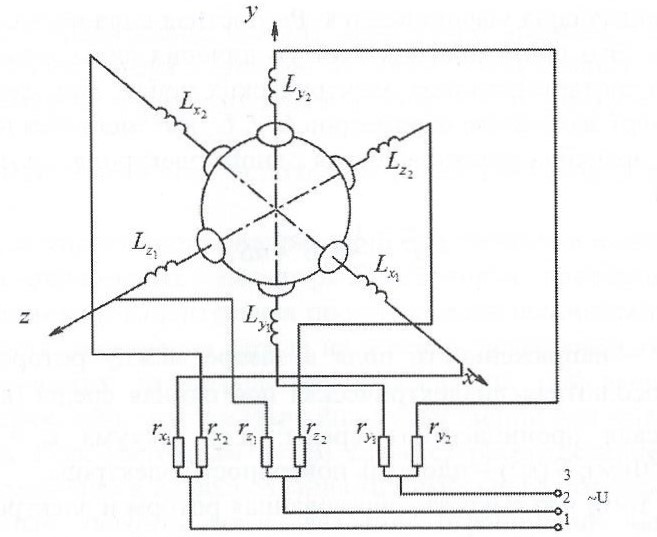
\includegraphics [scale=0.5] {sphere_susp_scheme}
  \caption{Расчетная конечно-элементная схема трехосного пассивного электростатического подвеса}
  \label{img:sphere_susp_scheme}
\end{figure}

Для задания в электромеханических элементах \textit{TRANS126} зависимости электрической емкости от величины зазора $C(\delta)$ построим вспомогательную модель и произведем расчет емкости с помощью макроса \textit{CMATRIX}. Вспомогательная модель представляет собой полость между фиксированными электродами цепи и ротором, заполненную электростатическими SOLID122 элементами. Как и в предыдущей главе, итерационно находим зависимость электрической емкости от величины зазора $C(\delta)$ и передаем значения в определение электромеханических элементов.